\chapter{Introduction to Matrices and Linear Systems}

Although the Earth System is well-known to be filled with non-linear processes, we still benefit from learning how to work with linear systems, as which many Earth Science problems can be approximated. This actually works well in a number of cases. For example, in Atmosphere Sciences, we often consider what is called a \textit{perturbation equation}, which assumes that variations from the mean state are small enough to neglect quadratic perturbed terms. \textit{Matrices} are one of the most fundamental objects in Linear Algebra, and we are going to address the basic aspects related to them in the first chapter.

\section{Definition and Operations of Matrices}

\subsection{Basic Structure of Matrices}
\index{Matrix}\keywordhl{Matrices} are rectangular arrays of numbers, which can be real or complex. For now we will work with real numbers, and defer the treatment about complex matrices to later chapters. A matrix having $m$ rows and $n$ columns is called an $m \times n$ matrix. A matrix with the same number of rows and columns, i.e.\ $m = n$, is called a \index{Matrix!Square Matrix}\keywordhl{square matrix}. Below shows some examples of matrices.

\begin{minipage}{0.5\textwidth}
$\begin{bmatrix}
1 & 2 & -2 & 5 \\
1 & 3 & \sqrt{3} & 7
\end{bmatrix}$\par\vspace{4pt}
A $2 \times 4$ real matrix.
\end{minipage}%
\begin{minipage}{0.5\textwidth}
$\begin{bmatrix}
2 - \imath \\
0 \\
1 \\
3 \imath
\end{bmatrix}$\par\vspace{4pt}
A $4 \times 1$ complex matrix.
\end{minipage}\\
\begin{minipage}{0.5\textwidth}
$\begin{bmatrix}
3 & 2 & 9 \\
-4 & 0 & 4 \\
5 & 2 & -3
\end{bmatrix}$\par\vspace{4pt}
A $3 \times 3$ real, square matrix.
\end{minipage}

Given any matrix $A$, its entry at row $i$ and column $j$ will be denoted as $A_{ij}$. For example,
\begin{align*}
& A =
\begin{tikzpicture}[baseline=-\the\dimexpr\fontdimen22\textfont2\relax]
\matrix(mymatrix)[matrix of math nodes, left delimiter={[}, 
right delimiter={]}, inner sep=3pt, ampersand replacement=\&]
{2 \& 1 \& 9 \\
\textcolor{red}{5} \& -3 \& 7 \\};
\node at (mymatrix-1-1)[above, font=\scriptsize, yshift=5, Green] {Col 1};
\node at (mymatrix-2-3)[right, font=\scriptsize, xshift=15, Green] {Row 2};
\draw [Green, dotted, fill=blue!50, fill opacity=0.2] (mymatrix-1-1.north west) rectangle (mymatrix-2-1.south east);
\draw [Green, dotted, fill=blue!50, fill opacity=0.2] (mymatrix-2-1.north west) rectangle (mymatrix-2-3.south east);
\end{tikzpicture}
& \textcolor{red}{A_{21} = 5}
\end{align*}
Short Exercise: Find $A_{13}$ and $A_{22}$.\footnote{$A_{13} = 9$, $A_{22} = -3$.}

\subsection{Matrix Operations} 
\subsubsection{Addition and Subtraction}
Addition and subtraction between two matrices $A$ and $B$ are carried out \textit{element-wise}, which means that if $C = A \pm B$, then $C_{ij} = A_{ij} \pm B_{ij}$. This implies that the two matrix operands must be of the same shape, and addition/subtraction is not possible for two matrices with different extents. For instance, if we have
\begin{align*}
A &=
\begin{bmatrix}
1 & 2 \\
3 & 4 \\
5 & 6
\end{bmatrix} &
B &= 
\begin{bmatrix}
1 & 1 \\
0 & 8 \\
1 & 7
\end{bmatrix}
\end{align*}
Then
\begin{align*}
A+B &= 
\begin{bmatrix}
1 & 2 \\
3 & 4 \\
5 & 6
\end{bmatrix}
+
\begin{bmatrix}
1 & 1 \\
0 & 8 \\
1 & 7
\end{bmatrix} \\
&= 
\begin{bmatrix}
1+1 & 2+1 \\
3+0 & 4+8 \\
5+1 & 6+7
\end{bmatrix} \\
&= 
\begin{bmatrix}
2 & 3 \\
3 & 12 \\
6 & 13
\end{bmatrix}
\end{align*}
Short Exercise: Find $A-B$.\footnote{$A-B = \begin{bmatrix}
0 & 1 \\
3 & -4 \\
4 & -1
\end{bmatrix}$}

\subsubsection{Scalar Multiplication} Multiplying a matrix by a constant constitutes a \index{Scalar Multiplication}\keywordhl{scalar multiplication}, in which all entries are multiplied by the scalar. It is illustrated in the example below.
\begin{align*}
A &= 
\begin{bmatrix}
2 & -5 & 6 \\
-1 & 4 & -3
\end{bmatrix} \\
3A &= 3
\begin{bmatrix}
2 & -5 & 6 \\
-1 & 4 & -3
\end{bmatrix} \\
&=
\begin{bmatrix}
3 \times 2 & 3 \times (-5) & 3 \times 6 \\
3 \times (-1) & 3 \times 4 & 3 \times (-3)
\end{bmatrix} \\
&=
\begin{bmatrix}
6 & -15 & 18 \\
-3 & 12 & -9
\end{bmatrix}
\end{align*}
Short Exercise: Find $\frac{1}{4}A$.\footnote{$A/4 = \begin{bmatrix}
1/2 & -5/4 & 3/2 \\
-1/4 & 1 & -3/4
\end{bmatrix}$}

\subsubsection{Matrix Multiplication/Matrix Product} Meanwhile, multiplication between two matrices, commonly referred to as \index{Matrix Product (Matrix Multiplication)}\keywordhl{matrix multiplication/matrix product}, is not element-wise. It can be only carried out if the number of columns of the first matrix equals to the number of rows of the second matrix, let's say $r$, in other words, they are of the shape $m \times r$ and $r \times n$ respectively. The resulting matrix is of the shape $m \times n$, which means that the number of rows/columns of the output matrix follows the first/second input matrix respectively. The following two examples explain this requirement.
\begin{align*}
& A = 
\begin{bmatrix}
1 & 2 & 2 \\
1 & 3 & 5
\end{bmatrix} &
& B = 
\begin{bmatrix}
1 \\
5 \\
7 
\end{bmatrix}
\end{align*}
Since the shapes of $A$ and $B$ are $2 \times 3$ and $3 \times 1$, the number of columns in $A$ and the number of rows in $B$ are both $3$, and hence matrix product between them is possible. The resulting matrix will be of size $2 \times 1$.
\begin{align*}
& C = 
\begin{bmatrix}
1 & 2 & 3 & 4 \\
2 & 0 & 6 & 1
\end{bmatrix} &
& D = 
\begin{bmatrix}
3 & 1\\
0 & 5\\
3 & 2
\end{bmatrix}
\end{align*}
As the number of columns in $C$ is 4, which is not equal to the number of rows in $D$, 3, matrix product is undefined in this case. Now we are ready to see how the entries in matrix product is exactly computed.

\begin{defn}[Matrix Product]
\label{defn:matprod}
Given an $m \times r$ matrix $A$ and an $r \times n$ matrix $B$, if we denote the matrix product between $A$ and $B$ as $C = AB$, then to calculate any entry in $C$ at row $i$ and column $j$, we select row $i$ from the first matrix $A$ and column $j$ from the second matrix $B$. Subsequently, take the products between the $r$ pairs of numbers from that row and column. Their sum will then be the required value of the entry, i.e.\
\begin{align*}
C_{ij} = (AB)_{ij} &= A_{i1}B_{ij} + A_{i2}B_{2j} + A_{i3}B_{3j} + ... + A_{ir}B_{rj} \\
&= \sum_{k=1}^{r} A_{ik}B_{kj}
\end{align*}
again, $r$ is the number of columns/rows in the first/second matrix.
\end{defn}
\begin{exmp}
Calculate the matrix product $C = AB$, where
\begin{align*}
& A = 
\begin{bmatrix}
\textcolor{red}{1} & \textcolor{red}{3} & \textcolor{red}{5} \\
2 & 4 & 6 
\end{bmatrix} &
& B = 
\begin{bmatrix}
1 & \textcolor{blue}{4} \\
2 & \textcolor{blue}{5} \\
3 & \textcolor{blue}{6}
\end{bmatrix}
\end{align*}
\end{exmp}
\begin{solution}
The output will be a $2 \times 2$ matrix. Using the definition, we have
\begin{align*}
C_{11} = (AB)_{11} &= A_{11}B_{11} + A_{12}B_{21} + A_{13}B_{31} \\
&= (1)(1) + (3)(2) + (5)(3) = 22 \\
C_{12} = (AB)_{12} &= \textcolor{red}{A_{11}}\textcolor{blue}{B_{12}} + \textcolor{red}{A_{12}}\textcolor{blue}{B_{22}} + \textcolor{red}{A_{13}}\textcolor{blue}{B_{32}} \\
&= \textcolor{red}{(1)}\textcolor{blue}{(4)} + \textcolor{red}{(3)}\textcolor{blue}{(5)} + \textcolor{red}{(5)}\textcolor{blue}{(6)} = 49
\end{align*}
Hence the entries along the first row of $C$ will be 22 and 49. The remaining entries at the second row are found in a similar way, and the readers are encouraged to do this themselves. You should be able to get
\begin{align*}
C = 
\begin{bmatrix}
22 & 49 \\
28 & 64
\end{bmatrix}   
\end{align*}
\end{solution}

Matrix product has some important properties, listed as follows.
\begin{proper}
\label{proper:matmul}
If $A$, $B$, $C$ are some matrices having compatible shapes so that the matrix multiplication operations below are valid, then
\begin{align*}
\underbrace{A\cdots A}_{k \text{ times}} &= A^k &\text{$k$-th power of a (square) matrix} \\
(AB)C &= A(BC) = ABC &\text{Associative Property} \\
(A \pm B)C &= AC \pm BC &\text{Distributive Property} \\
A(B \pm C) &= AB \pm AC &\text{Distributive Property}
\end{align*}
\end{proper}
Another important observation is that, in general $AB \neq BA$ even if the matrix products $AB$ and $BA$ are both well-defined, so they are not \textit{commutative}. However, as we will see later, there are some distinct exceptions of this.
\begin{exmp}
Calculate $-2A + 3B$, where
\begin{align*}
& A = 
\begin{bmatrix}
1 & 6 & 9 \\
4 & 4 & 6 
\end{bmatrix} &
& B = 
\begin{bmatrix}
4 & 8 & 6 \\
-5 & 0 & 3
\end{bmatrix}
\end{align*}
\end{exmp}
\begin{solution}
\begin{align*}
-2A + 3B &= 
-2\begin{bmatrix}
1 & 6 & 9 \\
4 & 4 & 6 
\end{bmatrix}
+3\begin{bmatrix}
4 & 8 & 6 \\
-5 & 0 & 3
\end{bmatrix} \\
&= \begin{bmatrix}
-2 & -12 & -18 \\
-8 & -8 & -12 
\end{bmatrix}
+ \begin{bmatrix}
12 & 24 & 18 \\
-15 & 0 & 9
\end{bmatrix} \\
&= \begin{bmatrix}
10 & 12 & 0 \\
-23 & -8 & -3
\end{bmatrix}
\end{align*}
\end{solution}

\begin{exmp}
Compute $(A+3B)(2A-B)$, where
\begin{align*}
& A = 
\begin{bmatrix}
1 & 2 \\
3 & 5 
\end{bmatrix} &
& B = 
\begin{bmatrix}
-2 & 0 \\
4 & -1
\end{bmatrix}
\end{align*}
\end{exmp}
\begin{solution}
Using distributive property in Properties \ref{proper:matmul}, the expression is equivalent to
\begin{align*}
(A+3B)(2A-B) &= A(2A-B) + (3B)(2A-B)\\
&= A(2A) + A(-B) + (3B)(2A) + (3B)(-B) \\
&= 2A^2 - AB + 6BA - 3B^2
\end{align*}
Bear in mind that $AB \neq BA$. We calculate each term, which gives
\begin{align*}
A^2 &=
\begin{bmatrix}
1 & 2 \\
3 & 5 
\end{bmatrix}
\begin{bmatrix}
1 & 2 \\
3 & 5 
\end{bmatrix} \\
&=
\begin{bmatrix}
(1)(1)+(2)(3) & (1)(2)+(2)(5) \\
(3)(1)+(5)(3) & (3)(2)+(5)(5) 
\end{bmatrix} \\
&=
\begin{bmatrix}
7 & 12 \\
18 & 31 
\end{bmatrix}
\end{align*}
\begin{align*}
AB &= 
\begin{bmatrix}
1 & 2 \\
3 & 5 
\end{bmatrix}
\begin{bmatrix}
-2 & 0 \\
4 & -1
\end{bmatrix} \\
&=
\begin{bmatrix}
(1)(-2)+(2)(4) & (1)(0)+(2)(-1) \\
(3)(-2)+(5)(4) & (3)(0)+(5)(-1) 
\end{bmatrix} \\
&= 
\begin{bmatrix}
6 & -2 \\
14 & -5 
\end{bmatrix}
\end{align*}
Similarly, it is not difficult to obtain
\begin{align*}
BA &= 
\begin{bmatrix}
-2 & -4 \\
1 & 3 
\end{bmatrix} &
B^2 &= 
\begin{bmatrix}
4 & 0 \\
-12 & 1 
\end{bmatrix} 
\end{align*}
Hence the final answer will be
\begin{align*}
2A^2 - AB + 6BA - 3B^2 &= 
2\begin{bmatrix}
7 & 12 \\
18 & 31 
\end{bmatrix}
-\begin{bmatrix}
6 & -2 \\
14 & -5 
\end{bmatrix}
+6\begin{bmatrix}
-2 & -4 \\
1 & 3 
\end{bmatrix}
-3\begin{bmatrix}
4 & 0 \\
-12 & 1 
\end{bmatrix} \\
&=
\begin{bmatrix}
14 & 24 \\
36 & 62 
\end{bmatrix}
-\begin{bmatrix}
6 & -2 \\
14 & -5 
\end{bmatrix}
+\begin{bmatrix}
-12 & -24 \\
6 & 18 
\end{bmatrix}
-\begin{bmatrix}
12 & 0 \\
-36 & 3 
\end{bmatrix} \\
&= 
\begin{bmatrix}
-16 & 2 \\
64 & 82 
\end{bmatrix}
\end{align*}
\end{solution}
Alternatively, one can evaluate $C = A+3B$ and $D = 2A-B$ first, and subsequently calculate the matrix dot product $CD$. (This is actually somehow easier.) The readers should try this as an exercise.

\subsubsection{Matrix Equation Manipulation}
For any matrix equation, one can do addition, subtraction and multiplication on both sides of the equation. However, one important note is that multiplying a matrix to an equation requires the matrix to be inserted to the left (or right) on both sides, respecting the order. So, for a matrix equation like (assuming the shapes are compatible),
\begin{align*}
AB-C = DE+F
\end{align*}
if we want to take the product with a matrix $G$, then it can be
\begin{align*}
G(AB-C) &= G(DE+F) \\
(AB-C)G &= (DE+F)G
\end{align*}
but we have, in general
\begin{align*}
G(AB-C) &\neq (DE+F)G \\
(AB-C)G &\neq G(DE+F)
\end{align*}
Taking successive matrix products follows the same principle, step by step. Using the example above, for another matrix $H$, we note some possible outcomes.
\begin{align*}
HG(AB-C) &= HG(DE+F) \\
(AB-C)GH &= (DE+F)GH \\
G(AB-C)H &= G(DE+F)H 
\end{align*}
However, be careful that cancellation at both sides may not be correct. If $AB = AC$, then we cannot conclude that $B = C$ for sure, although it is not impossible (and happens quite often).

\section{Definition of Linear Systems of Equations}
\label{section:deflinsys}
The prime application of matrices is to deal with \index{Linear System of Equations}\keywordhl{linear systems (of equations)}. To understand what a linear system is, we first have to know the definition of a \index{Linear Equation}\keywordhl{linear equation} (possibly in multiple variables, let's say $x_1$, $x_2$, $\ldots$). For a linear equation, in any additive term, there is at most one variable or unknown, with a power of one, like $3x_1$, $-x_2$. This means that there are no cross-product terms such as $2x_1x_2$, variables with a power that is not one, like $x_1^3$, or non-linear functions, including $\sin{x_1}, e^{x_2}$. For $n$ variables, a linear equation has the following definition.
\begin{defn}[Linear Equation]
A linear equation has the form of
\begin{align*}
\sum_{j=1}^n a_jx_j = a_1x_1 + a_2x_2 + a_3x_3 + \cdots + a_nx_n = h
\end{align*}
where $x_1, x_2, \ldots$ are the unknowns, while $a_1, a_2, \ldots$ and $h$ are some constants. If $h = 0$, then it is known as a \index{Linear Equation!Homogeneous Linear Equation}\keywordhl{homogeneous linear equation}.
\end{defn}
Short Exercise: Determine whether the equations below are (a) linear, and if they are linear, then (b) homogeneous or not.\footnote{Linear/Inhomogeneous, Non-linear, Linear/Inhomogeneous, Non-linear, Linear/Homogeneous, Non-linear.}
\begin{enumerate}
    \item $3x + 4y = 5$ 
    \item $\cos x + \ln y = 0$
    \item $7x - 5z = 2$ 
    \item $x^2 + y^{-3/2} = 1$
    \item $x + 3y + 6z = 0$
    \item $xyz = 8$ 
\end{enumerate}
A system of linear equations are then simply a family of $m$ linear equations, $m \geq 1$.
\begin{defn}[Linear System of Equations]
\label{defn:linsys}
A linear system of size $m \times n$ has the form of
\begin{equation*}
\begin{cases}
\sum_{j=1}^n a_j^{(1)}x_j = a_1^{(1)}x_1 + a_2^{(1)}x_2 + a_3^{(1)}x_3 + \cdots + a_n^{(1)}x_n &= h^{(1)} \\
\sum_{j=1}^n a_j^{(2)}x_j = a_1^{(2)}x_1 + a_2^{(2)}x_2 + a_3^{(2)}x_3 + \cdots + a_n^{(2)}x_n &= h^{(2)} \\
\vdots \\
\sum_{j=1}^n a_j^{(m)}x_j = a_1^{(m)}x_1 + a_2^{(m)}x_2 + a_3^{(m)}x_3 + \cdots + a_n^{(m)}x_n &= h^{(m)} \\
\end{cases}   
\end{equation*}
If $h^{(1)}, h^{(2)}, \ldots$ at the right hand side are all zeros, then the system is called a \index{Linear System of Equations!Homogeneous Linear System of Equations}\keywordhl{homogeneous linear system (of equations)}. It is not hard to see that for any homogeneous linear system, it always has a trivial solution of $x_j = 0$ for $j = 1, \ldots, n$, or expressed as $\vec{x} = \textbf{0}$. However, such trivial solution may not be the only solution to the system, as we shall see in !???.
\end{defn}
Below shows some examples of linear systems.
\begin{flalign*}
&\begin{cases}
3x + 4y &= 5 \\
7x + 9y &= 13
\end{cases}&   
\end{flalign*}
A $2 \times 2$ linear system with two equations, two unknowns.
\begin{flalign*}
&\begin{cases}
x + 2y - 4z &= 3 \\
x - y + 3z &= -4
\end{cases}&   
\end{flalign*}
A $2 \times 3$ linear system with two equations, three unknowns.
\begin{flalign*}
&\begin{cases}
x + 2y + 3z &= 0 \\
2x + 3z &= 0 \\
4x - 5y &= 0
\end{cases}&  
\end{flalign*}
A $3 \times 3$ homogeneous linear system (homogeneous as the R.H.S. are all zeros), notice the coefficients for some unknowns in some equations are zeros as well, e.g.\ in the second equation $y$ has a coefficient of zero and does not appear.\\

The above formulation of a linear system closely resembles a tabular structure. Therefore, we are motivated to represent such systems with the language of matrices. Indeed, it is possible to rewrite an $m \times n$ linear system as $A\vec{x} = \vec{h}$, where $A$ is an $m \times n$ matrix with entries copied from the coefficients in front of the variables arranged like those in Definition \ref{defn:linsys}. In this book sometimes we will call it a \index{Matrix!Coefficient Matrix}\textit{coefficient matrix}. Meanwhile, $\vec{x}$ is a column vector (an $n \times 1$ matrix) holding the $n$ unknowns, and $\vec{h}$ is another column vector (an $m \times 1$ matrix) that contains the $m$ constants at the right hand side of the linear system.
\begin{proper}
\label{proper:linsysmat}
For a linear system like that in Definition \ref{defn:linsys}, it can be rewritten as $A\vec{x} = \vec{h}$, where $A_{ij} = a_{j}^{(i)}$, $\vec{x} = x_j$, and $\vec{h} = h^{(i)}$.
\end{proper}
Using the second example above as an illustration, we can easily verify that
\begin{equation*}
\begin{cases}
x + 2y - 4z &= 3 \\
x - y + 3z &= -4
\end{cases}   
\end{equation*}
can be expressed as (you should check it yourself)
\begin{align*}
\begin{bmatrix}
1 & 2 & -4 \\
1 & -1 & 3 
\end{bmatrix}
\begin{bmatrix}
x \\
y \\
z
\end{bmatrix}
=
\begin{bmatrix}
3 \\
-4
\end{bmatrix}
\end{align*}
An even simpler representation is the \index{Matrix!Augmented Matrix}\keywordhl{augmented matrix} which omits the unknowns and concatenates the remaining matrices.
\begin{equation*}
\left[\begin{array}{@{}ccc|c@{}}
1 & 2 & -4 & 3\\
1 & -1 & 3 & -4
\end{array}\right]
\end{equation*}

\section{Elementary Row Operations}
When we construct a matrix, it is natural to think about how to utilize its structure. \index{Elementary Row Operations}\keywordhl{Elementary row operations} provide such possibility in three ways, outlined in the following definition.
\begin{defn}[Elementary Row Operations]
\label{defn:elerowop}
The three types of elementary row operations are
\begin{enumerate}
\item Multiplying a row $R_{p}$ by any constant $c \neq 0$.
\item Adding a row $R_{q}$ times any constant $c \neq 0$, to another row $R_{p}$, such that the new row becomes $R_{p} + cR_{q}$
\item Swapping a row $R_{p}$ with another row $R_{q}$.
\end{enumerate}
To facilitate the operations, we mark these three actions using the following notations.
\begin{enumerate}
\item $cR_{p} \rightarrow R_{p}$,
\item $R_{p} + cR_{q} \rightarrow R_{p}$,
\item $R_{p} \leftrightarrow R_{q}$
\end{enumerate}
\end{defn}
For example, the matrix $A$
\begin{equation*}
\begin{bmatrix}
1 & 2 & 3 \\
5 & 7 & 11
\end{bmatrix}
\end{equation*}
can be transformed to a new matrix $A'$
\begin{equation*}
\begin{bmatrix}
1 & 2 & 3 \\
3 & 3 & 5
\end{bmatrix}
\end{equation*}
if we apply the elementary row operation, subtracting $2R_1$ from $R_2$  (i.e.\ $R_2 - 2R_1 \to R_2$). \\Short Exercise: Find out the resulting matrix $A''$ if we multiply the first row of $A'$ by $3$ and then subtract the second row from the first row.\footnote{
$\begin{bmatrix}
0 & 3 & 4 \\
3 & 3 & 5
\end{bmatrix}$}\\

Attentive readers may have noticed that these three operations are what we have been always doing to equations when solving a linear system, as taught in high school. We re-introduce them as elementary row operations here first as they are fundamental to the treatment of later chapters.

\section{Earth Science Applications}
\label{sec:ch1earth}
\begin{exmp}
\label{exmp:seismic1}
Seismic wave follows \textit{Snell's Law} like a light ray when it comes to refraction. Assuming the ground can be modelled as a two-layer system (see Figure \ref{fig:seismic1}), and we know a particular train of seismic wave generated from an underground source that reaches the ground receiver travels at an angle of $\theta_1 = \SI{45}{\degree}$/$\theta_2 = \SI{60}{\degree}$ to the vertical at the top/bottom layer. Given that the horizontal and vertical distance between the seismic source and the surface receiver are $d = \SI{1200}{\m}$ and $h = \SI{800}{\m}$. Construct a linear system for this situation in two unknowns: the depth of the top layer $y$ and the horizontal displacement $x$ (in meters) where the wave reaches at the interface relative to the source.
\end{exmp}
\begin{figure}
\centering
\begin{tikzpicture}
    \draw [black, bottom color=brown!50!orange, top color=orange!50] (0,-0.4) rectangle (8,2.4);
    \draw [black, bottom color=brown!50, top color=brown!10] (0,2.4) rectangle (8,4);
    \coordinate (source) at (1,0);
    \draw [red] (source) circle (0.1);
    \draw [red] (source) circle (0.2);
    \draw [red] (source) circle (0.3);
    \coordinate (interface) at (5.4,2.4);
    \coordinate (receive) at (7,4);
    \draw [black, fill] (6.9,4) rectangle (7.1,4.4);
    \draw [thick, dotted] (interface) -- ++ (0,1) node (interup){};
    \draw [thick, dotted] (interface) -- ++ (0,-1) node (interdown){};
    \draw [red, thick] (source) -- (interface);
    \draw [red, thick, ->] (interface) -- (receive);
    \pic [draw, "$\theta_2 = \SI{60}{\degree}$", angle eccentricity=2, font=\scriptsize, pic text options={xshift=-2}] {angle = source--interface--interdown};
    \pic [draw, "$\theta_1 = \SI{45}{\degree}$", angle eccentricity=2.5, font=\scriptsize, pic text options={xshift=2}] {angle = receive--interface--interup};
    \draw [blue, thick, <->] (7,2.4) -- (7,4) node[below, sloped, midway]{$y$};
    \draw [thick, <->] (8.2,0) -- (8.2,4) node[below, sloped, midway]{$h = \SI{800}{\m}$};
    \draw [blue, thick, <->] (1,2.3) -- (5.4,2.3) node[below, sloped, midway]{$x$};
    \draw [thick, <->] (1,-0.6) -- (7,-0.6) node[below, sloped, midway]{$d = \SI{1200}{\m}$};
\end{tikzpicture}
\caption{The underground schematic for the seismic ray in Example \ref{exmp:seismic1}.}
\label{fig:seismic1}
\end{figure}
\begin{solution}
We can deduce two equations from the given information. Consider the upper portion of the seismic ray, from basic trigonometry, we know that 
\begin{align*}
\frac{d-x}{y} &= \tan \theta_1 \\
d-x &= (\tan\theta_1) y \\
x + (\tan\theta_1) y &= d
\end{align*}
Similarly, for the lower portion of the seismic ray, we have
\begin{align*}
\frac{x}{h-y} &= \tan \theta_2 \\
x &= (\tan \theta_2) h - (\tan\theta_2) y \\
x + (\tan\theta_2) y &= (\tan \theta_2) h
\end{align*}
The corresponding linear system is
\begin{align*}
\begin{cases}
x + (\tan\theta_1) y &= d \\
x + (\tan\theta_2) y &= (\tan \theta_2) h
\end{cases}
\end{align*}
where $x$ and $y$ are the unknowns to be solved. $d$, $h$, $\theta_1$ and $\theta_2$ (and hence $\tan\theta_1$ and $\tan\theta_2$) are constants. Expressing the system in matrix form, we have
\begin{align*}
\begin{bmatrix}
1 & \tan\theta_1 \\
1 & \tan\theta_2
\end{bmatrix}
\begin{bmatrix}
x \\
y
\end{bmatrix}
=
\begin{bmatrix}
d \\
(\tan \theta_2) h
\end{bmatrix}
\end{align*}
Substituting the provided values for the constants ($\tan\theta_1 = \tan(\SI{45}{\degree}) = 1$, $\tan\theta_2 = \tan(\SI{60}{\degree}) = \sqrt{3}$), we have
\begin{align*}
\begin{bmatrix}
1 & 1 \\
1 & \sqrt{3}
\end{bmatrix}
\begin{bmatrix}
x \\
y
\end{bmatrix}
=
\begin{bmatrix}
1200 \\
800\sqrt{3}
\end{bmatrix}
\end{align*}
\end{solution}

\begin{exmp}
\label{exmp:multilayer1}
The radiation transfer across the atmosphere of any planet (including the Earth) in the Solar system can be compared to a \textit{multi-layer model} with fully absorbing layers (note that it is just a simplistic approach). Assume there are $N$ such layers and the total rate of incident Solar radiation reaching the surface is $E_{in}$. Each of the layers also emits radiation to the other layers directly above/below itself. The rate of emission for the $j$-th layer that has a temperature $T_j$ is $E_j = \sigma T_j^4$ according to the \textit{Stefan–Boltzmann Law}, with $\sigma = \SI{5.67e-8}{\W \per \square\m \per \quartic\K}$. The overall scenario can be seen in Figure \ref{fig:multilayer1}. Formulate a linear system that represents the energy equilibrium (incoming radiation = outgoing radiation) of all layers and the surface, with $E_j$ being the unknowns, over $j = 1, 2, \ldots, N, N+1$.
\end{exmp}
\begin{figure}
\centering
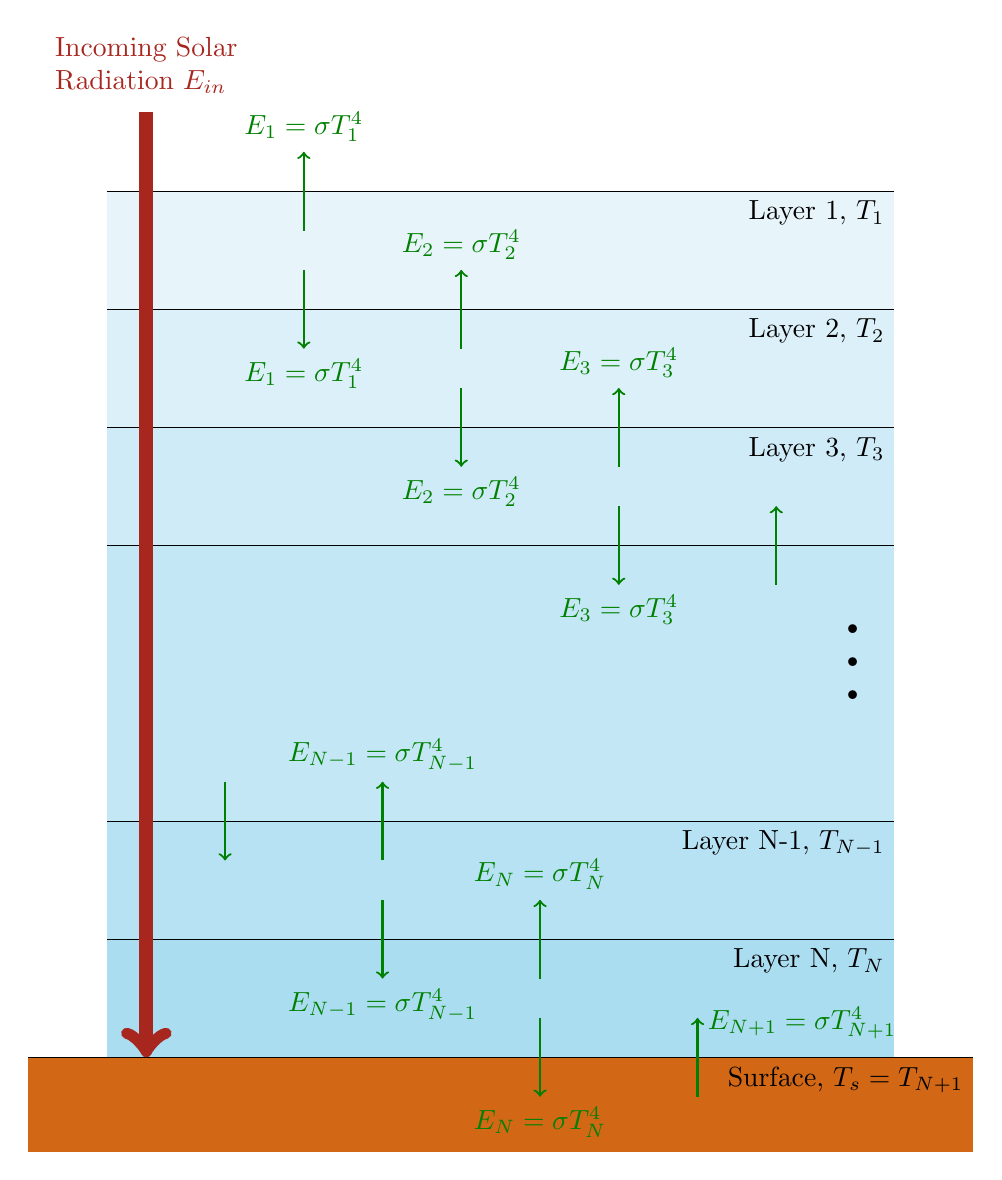
\begin{tikzpicture}
    \fill [SkyBlue!70] (0,0) rectangle (10, 1.5) node[below left, black]{Layer N, $T_N$};
    \fill [SkyBlue!60] (0,1.5) rectangle (10, 3) node[below left, black]{Layer N-1, $T_{N-1}$};
    \fill [SkyBlue!50] (0,3) rectangle (10, 6.5) node[below left, black, scale=3]{$\vdots$};
    \fill [SkyBlue!40] (0,6.5) rectangle (10, 8) node[below left, black]{Layer 3, $T_3$};
    \fill [SkyBlue!30] (0,8) rectangle (10, 9.5) node[below left, black]{Layer 2, $T_2$};
    \fill [SkyBlue!20] (0,9.5) rectangle (10, 11) node[below left, black]{Layer 1, $T_1$};
    \fill [Brown!50!Orange] (-1,-1.2) rectangle (11, 0) node[below left, black]{Surface, $T_s = T_{N+1}$};
    \draw [black] (-1,0) -- (11,0) ;
    \draw [black] (0,1.5) -- (10,1.5);
    \draw [black] (0,3) -- (10,3);
    \draw [black] (0,6.5) -- (10,6.5);
    \draw [black] (0,8) -- (10,8);
    \draw [black] (0,9.5) -- (10,9.5);
    \draw [black] (0,11) -- (10,11);
    \draw [Mahogany, ->, line width=5pt] (0.5,12) -- (0.5,0) node[align=left, pos=-0.05]{Incoming Solar\\ Radiation $E_{in}$};
    \draw [Green, thick, ->] (2.5,10.5) -- (2.5,11.5) node[above]{$E_1 = \sigma T_1^4$};
    \draw [Green, thick, ->] (2.5,10) -- (2.5,9) node[below]{$E_1 = \sigma T_1^4$};
    \draw [Green, thick, ->] (4.5,9) -- (4.5,10) node[above]{$E_2 = \sigma T_2^4$};
    \draw [Green, thick, ->] (4.5,8.5) -- (4.5,7.5) node[below]{$E_2 = \sigma T_2^4$};
    \draw [Green, thick, ->] (6.5,7.5) -- (6.5,8.5) node[above]{$E_3 = \sigma T_3^4$};
    \draw [Green, thick, ->] (6.5,7) -- (6.5,6) node[below]{$E_3 = \sigma T_3^4$};
    \draw [Green, thick, ->] (8.5,6) -- (8.5,7);
    \draw [Green, thick, ->] (3.5,2.5) -- (3.5,3.5) node[above]{$E_{N-1} = \sigma T_{N-1}^4$};
    \draw [Green, thick, ->] (3.5,2) -- (3.5,1) node[below]{$E_{N-1} = \sigma T_{N-1}^4$};
    \draw [Green, thick, ->] (5.5,1) -- (5.5,2) node[above]{$E_N = \sigma T_N^4$};
    \draw [Green, thick, ->] (5.5,0.5) -- (5.5,-0.5) node[below]{$E_N = \sigma T_N^4$};
    \draw [Green, thick, ->] (7.5,-0.5) -- (7.5,0.5) node[above right, pos=0.6]{$E_{N+1} = \sigma T_{N+1}^4$};
    \draw [Green, thick, ->] (1.5,3.5) -- (1.5,2.5);
\end{tikzpicture}
\caption{The atmospheric profile with multiple ($N$) absorbing layers in Example \ref{exmp:multilayer1}. The surface is treated as an extra $N$+1-th layer.}
\label{fig:multilayer1}
\end{figure}
\begin{solution}
Considering the energy equilibrium for the first (topmost) layer, we have
\begin{align*}
-2E_1 + E_2 = 0 
\end{align*}
Going down to the second layer, it is
\begin{align*}
E_1 - 2E_2 + E_3 = 0
\end{align*}
In general, for the $j$-th layer in the middle, where $j$ runs from $2$ to $N$, we can similarly obtain
\begin{align*}
E_{j-1} - 2E_j + E_{j+1} = 0
\end{align*}
Finally, for the surface (the $N+1$-th layer), we have
\begin{align*}
E_N - E_{N+1} + E_{in} &= 0 \\
E_N - E_{N+1} &= -E_{in} 
\end{align*}
Summarizing all the $N+1$ equations, they can be expressed in matrix form as
\begin{align*}
\begin{bmatrix}
-2 & 1 & 0 & \cdots & 0 & 0 & 0 \\
1 & -2 & 1 & & 0 & 0 & 0 \\
0 & 1 & -2 & & 0 & 0 & 0 \\
\vdots & & & \ddots & & & \vdots \\
0 & 0 & 0 & & -2 & 1 & 0 \\
0 & 0 & 0 & & 1 & -2 & 1 \\
0 & 0 & 0 & \cdots & 0 & 1 & -1
\end{bmatrix}
\begin{bmatrix}
E_1 \\
E_2 \\
E_3 \\
\vdots \\
E_{N-1} \\
E_N \\
E_{N+1}
\end{bmatrix}
=
\begin{bmatrix}
0 \\
0 \\
0 \\
\vdots \\
0 \\
0 \\
-E_{in}
\end{bmatrix}
\end{align*}
Particularly, for $N=4$, it is
\begin{align*}
\begin{bmatrix}
-2 & 1 & 0 & 0 & 0 \\
1 & -2 & 1 & 0 & 0 \\
0 & 1 & -2 & 1 & 0 \\
0 & 0 & 1 & -2 & 1 \\
0 & 0 & 0 & 1 & -1
\end{bmatrix}
\begin{bmatrix}
E_1 \\
E_2 \\
E_3 \\
E_4 \\
E_5
\end{bmatrix}
=
\begin{bmatrix}
0 \\
0 \\
0 \\
0 \\
-E_{in}
\end{bmatrix}
\end{align*}
\end{solution}
We will talk about how to solve the linear systems in these two examples in Section \ref{sec:ch3earth}.

\section{Python Programming}
We will use the package \texttt{numpy} and \texttt{scipy} throughout the book to solve linear algebra problems via \textit{Python} programming. First, we can define a 2D \texttt{numpy} array that works as a matrix.
\begin{lstlisting}
import numpy as np
myMatrix1 = np.array([[1, 4], [5, 3]])
print(myMatrix1)
\end{lstlisting}
which gives
\begin{lstlisting}
[[1 4]
 [5 3]]
\end{lstlisting}
representing the matrix
\begin{align*}
\begin{bmatrix}
1 & 4 \\
5 & 3
\end{bmatrix}
\end{align*}
We can similarly define another matrix
\begin{lstlisting}
myMatrix2 = np.array([[1, 3], [5, 6]])    
\end{lstlisting}
Addition, subtraction, and scalar multiplication are straight-forward.
\begin{lstlisting}
myMatrix3 = 3*myMatrix1 - 4*myMatrix2
print(myMatrix3)
\end{lstlisting}
The above code produces
\begin{lstlisting}
[[ -1   0]
 [ -5 -15]]
\end{lstlisting}
and you can verify the answer by hand. Meanwhile, matrix product is done by the function \texttt{np.matmul()}.
\begin{lstlisting}
myMatrix4 = np.matmul(myMatrix1, myMatrix2) # or equivalently myMatrix1 @ myMatrix2
print(myMatrix4)
\end{lstlisting}
gives
\begin{lstlisting}
[[21 27]
 [20 33]]
\end{lstlisting}
To select a specfic entry, use indexing by square brackets. The first index/second index represents row/column. Beware that each index starts at zero in \textit{Python}. So putting the number $1$ in the first/second index actually means the second row/column. So
\begin{lstlisting}
print(myMatrix4[1,0])
\end{lstlisting}
refers to the entry at row $2$, column $1$ of \verb|myMatrix4| which is $20$. Also, we can select the $i$-th row (or the $j$-th column) by \verb|<Matrix>[i-1, :]| (\verb|<Matrix>[:, j-1]|), where the colon \verb|:| implies selecting along the entire row (column). For example,
\begin{lstlisting}
print(myMatrix3[0,:])
print(myMatrix4[:,1])
\end{lstlisting}
gives
\verb|[-1  0]| and \verb|[27 33]| respectively. Now let's see how to perform elementary row operations. It will be easier and less error-prone if we copy the array before performing the operations.
\begin{lstlisting}
myMatrix5 = np.copy(myMatrix4)
myMatrix5[0,:] = myMatrix5[0,:]/3
print(myMatrix5)
\end{lstlisting}
The lines above, when executed, divide the second row of \verb|myMatrix5| (which is a copy of \verb|myMatrix4|) by $3$, and give
\begin{lstlisting}
[[ 7  9]
 [20 33]]    
\end{lstlisting}
Meanwhile, the subsequent lines below
\begin{lstlisting}
myMatrix5[1,:] = myMatrix5[1,:] - 2*myMatrix5[0,:]
print(myMatrix5)
\end{lstlisting}
proceed to subtract $2$ times the first row from the second row, and produce
\begin{lstlisting}
[[ 7  9]
 [ 6 15]]
\end{lstlisting}
Row interchange is a bit more tricky.
\begin{lstlisting}
myMatrix6 = np.copy(myMatrix4)
myMatrix6[[0, 1],:] = myMatrix6[[1, 0],:]    
\end{lstlisting}
This swaps the first and second row. (You can swap columns in a similar way.) Printing out the new matrix by \verb|print(myMatrix6)| shows
\begin{lstlisting}
[[20 33]
 [21 27]]
\end{lstlisting}
\textcolor{red}{An important pitfall is that, since our inputs to \texttt{np.array} are all integers, the previous arrays will automatically have a data type of \texttt{int} (integer). This may produce unexpected errors when the calculation leads to decimals/fractions.} If it is the case, then we can avoid such bugs by declaring the array with the keyword \verb|dtype=float| to use \textit{floating point numbers}, like
\begin{lstlisting}
myMatrix1 = np.array([[1, 4], [5, 3]], dtype=float) 
\end{lstlisting}
when printed out via \verb|print(myMatrix1)| it gives
\begin{lstlisting}
[[1. 4.]
 [5. 3.]]    
\end{lstlisting}
Notice the newly appeared decimal points after the original integers. Alternatively, we can add decimal points to the integer entries during the array declaration, as
\begin{lstlisting}
myMatrix1 = np.array([[1., 4.], [5., 3.]]) 
\end{lstlisting}

\section{Exercises}
\begin{Exercise}
Let 
\begin{align*}
& A =
\begin{bmatrix}
1 & 2 \\
5 & -1 \\
\end{bmatrix}
& B =
\begin{bmatrix}
-4 & 3 \\
-2 & 7 \\
\end{bmatrix}
\end{align*}
Find:
\begin{enumerate}[label=(\alph*)]
\item $A+B$,
\item $2A-\frac{3}{2}B$,
\item $AB$,
\item $BA$.
\end{enumerate}
\end{Exercise}
\begin{Answer}
\begin{enumerate}[label=(\alph*)]
\item $\begin{bmatrix}
-3 & 5 \\
3 & 6 \\
\end{bmatrix}$
\item $\begin{bmatrix}
8 & -\frac{1}{2} \\
13 & -\frac{25}{2} \\
\end{bmatrix}$
\item $\begin{bmatrix}
-8 & 17 \\
-18 & 8 \\
\end{bmatrix}$
\item $\begin{bmatrix}
11 & -11 \\
33 & -11 \\
\end{bmatrix}$
\end{enumerate}   
\end{Answer}

\begin{Exercise}
Let 
\begin{align*}
& A =
\begin{bmatrix}
0 & 1 \\
3 & -1 \\
4 & 2 \\
\end{bmatrix}
& B =
\begin{bmatrix}
-1 & 0 & -2 \\
-2 & 1 & 3 \\
\end{bmatrix}
\end{align*}
Find:
\begin{enumerate}[label=(\alph*)]
\item $AB$,
\item $BA$.
\end{enumerate}
\end{Exercise}
\begin{Answer}
\begin{enumerate}[label=(\alph*)]
\item $\begin{bmatrix}
-2 & 1 & 3 \\
-1 & -1 & -9 \\
-8 & 2 & -2 \end{bmatrix}$
\item $\begin{bmatrix}
-8 & -5 \\
15 & 3
\end{bmatrix}$
\end{enumerate}
\end{Answer}

\begin{Exercise}
Let
\begin{align*}
A &=
\begin{bmatrix}
4 & 6\\
3 & 3
\end{bmatrix} \\
B &= 
\begin{bmatrix}
2 & 0\\
1 & 2
\end{bmatrix} \\
C &= 
\begin{bmatrix}
3 & 9 & 1\\
4 & 3 & -1
\end{bmatrix}
\end{align*}
Find:
\begin{enumerate}[label=(\alph*)]
\item $(A+B)C$,
\item $AC+BC$,
\item $(AB)C$,
\item $A(BC)$.
\end{enumerate}
\end{Exercise}
\begin{Answer}
\begin{enumerate}[label=(\alph*)]
\item $\begin{bmatrix}
42 & 72 & 0 \\ 
32 & 51 & -1 \\
\end{bmatrix}$
\item Same as above
\item $\begin{bmatrix}
90 & 162 & 2 \\
51 & 99 & 3
\end{bmatrix}$
\item Same as above
\end{enumerate}
\end{Answer}

\begin{Exercise}
Let 
\begin{align*}
& A =
\begin{bmatrix}
1 & 2 & 4\\
1 & 3 & 9\\
7 & 2 & -1
\end{bmatrix}
& B =
\begin{bmatrix}
1 & 5 & -2\\
4 & 3 & 1\\
0 & 2 & 3
\end{bmatrix}
\end{align*}
Find:
\begin{enumerate}[label=(\alph*)]
\item $(A+B)(2A-B)$,
\item $(\frac{3}{2}A - B)(-A + \frac{1}{2}B)$.
\end{enumerate}
\end{Exercise}
\begin{Answer}
\begin{enumerate}[label=(\alph*)]
\item $\begin{bmatrix}
16 & 23 & 129 \\
133 & 33 & 102 \\
27 & 9 & 128
\end{bmatrix}$
\item $\begin{bmatrix}
-\frac{233}{4} & -\frac{19}{4} & \frac{69}{2} \\
-\frac{339}{4} & -16 & 31 \\
\frac{109}{4} & \frac{33}{4} & -\frac{289}{4} \\
\end{bmatrix}$
\end{enumerate}
\end{Answer}

\begin{Exercise}
Let 
\begin{align*}
& A =
\begin{bmatrix}
1 & 0 & 3\\
2 & 1 & 6\\
5 & 2 & 0
\end{bmatrix}
& B =
\begin{bmatrix}
2 & 3 & 5\\
1 & 3 & 8\\
4 & 0 & 7
\end{bmatrix}
\end{align*}
Find:
\begin{enumerate}[label=(\alph*)]
\item $A^2$,
\item $B^2$,
\item $AB$, 
\item $BA$.
\end{enumerate}
\end{Exercise}
\begin{Answer}
\begin{enumerate}[label=(\alph*)]
\item $\begin{bmatrix}
16 & 6 & 3 \\
34 & 13 & 12 \\
9 & 2 & 27
\end{bmatrix}$
\item $\begin{bmatrix}
27 & 15 & 69 \\
37 & 12 & 85 \\
36 & 12 & 69 \\
\end{bmatrix}$
\item $\begin{bmatrix}
14 & 3 & 26 \\
29 & 9 & 60 \\
12 & 21 & 41
\end{bmatrix}$
\item $\begin{bmatrix}
33 & 13 & 24 \\
47 & 19 & 21 \\
39 & 14 & 12
\end{bmatrix}$
\end{enumerate}    
\end{Answer}

\begin{Exercise}
Let 
\begin{align*}
& A =
\begin{bmatrix}
1 & 1 \\
-1 & 1
\end{bmatrix}
& B =
\begin{bmatrix}
-1 & 1 \\
-1 & -1
\end{bmatrix}
\end{align*}
Show that $AB = BA$ in this case.
\end{Exercise}
\begin{Answer}
\begin{align*}
AB = BA = \begin{bmatrix}
-2 & 0 \\
0 & -2
\end{bmatrix} 
\end{align*}
\end{Answer}

\begin{Exercise}
Rewrite the following system of linear equations into matrix form.
\begin{equation*}
\begin{cases}
3y - 4z &= 6\\
5x - y + 2z &= 13\\
6x + z &= 8
\end{cases}
\end{equation*}
\end{Exercise}
\begin{Answer}
\begin{align*}
\begin{bmatrix}
0 & 3 & -4 \\
5 & -1 & 2 \\
6 & 0 & 1
\end{bmatrix}
\begin{bmatrix}
x \\
y \\
z
\end{bmatrix}
=
\begin{bmatrix}
6 \\ 
13 \\
8
\end{bmatrix}    
\end{align*}
or
\begin{align*}
\left[\begin{array}{@{}ccc|c@{}}
0 & 3 & -4 & 6 \\
5 & -1 & 2 & 13 \\
6 & 0 & 1 & 8
\end{array}\right]    
\end{align*}
\end{Answer}

\begin{Exercise}
For the following matrix,
\[
\begin{bmatrix}
2 & 3 & 5 & 7\\
1 & 2 & 4 & 8\\
1 & 3 & 6 & 10
\end{bmatrix}
\]
Find the results if the following elementary row operations are applied on it: 
\begin{enumerate}[label=(\alph*)]
\item Multiplying the third row by 2, and then subtracting the third row by the second row,
\item Adding the first row by 3 times the third row, and then interchanging the first and second row.\\
\end{enumerate}
\end{Exercise}
\begin{Answer}
\begin{enumerate}[label=(\alph*)]
\item $\begin{bmatrix}
2 & 3 & 5 & 7 \\
1 & 2 & 4 & 8 \\
1 & 4 & 8 & 12
\end{bmatrix}$
\item $\begin{bmatrix}
1 & 2 & 4 & 8 \\
5 & 12 & 23 & 37 \\
1 & 3 & 6 & 10\\
\end{bmatrix}$
\end{enumerate}
\end{Answer}

\begin{Exercise}
For the following matrix,
\[
\begin{bmatrix}
3 & 0 & 4 & 6 & 9\\
5 & 3 & 8 & -1 & 3 \\
2 & 5 & 4 & 3 & -7
\end{bmatrix}
\]
Find the elementary row operations needed to reduce the matrix to
\[
\begin{bmatrix}
1 & \frac{5}{2} & 2 & \frac{3}{2} & -\frac{7}{2} \\
5 & \frac{21}{2} & 10 & -\frac{5}{2} & -\frac{33}{2} \\
3 & 0 & 4 & 6 & 9
\end{bmatrix}
\]
\end{Exercise}
\begin{Answer}
\begin{enumerate}
\item Interchange Row $1$ and Row $3$ ($R_1 \leftrightarrow R_3$),
\item Multiply Row $1$ by $\frac{1}{2}$ ($\frac{1}{2}R_1 \rightarrow R_1$),
\item Subtract Row $3$ from Row $2$ ($R_2 - R_3 \rightarrow R_2$),
\item Add $3$ times Row $1$ to Row $2$ ($R_2 + 3R_1 \rightarrow R_2$).
\end{enumerate}
The order of step 1 and 2, as well as step 3 and 4, can be interchanged.
\end{Answer}

\begin{Exercise}
\label{ex:lapse}
The \textit{dry adiabatic lapse rate}, which is the rate of decrease in air temperature when an unsaturated air parcel rises, is about $\Gamma_{dry} = \SI{9.8}{\celsius \per \km}$. When the temperature of the air parcel falls below the \textit{dew point}, the air saturates and condensation occurs. Typically, dew point temperature of an air parcel will decrease at a rate of roughly $\Gamma_{dew} = \SI{2}{\celsius \per \km}$. Now, an air parcel with an initial air temperature/dew point temperature of $T_{a,ini} = \SI{25.4}{\celsius}$ / $T_{dew, ini} = \SI{17.8}{\celsius}$ at the ground starts to rise. Let $z_{cd}$ and $T_{cd}$ be the height above the ground (in \si{\km}) and temperature (in \si{\celsius}) of the air parcel when condensation occurs. Construct a linear system with $z_{cd}$ and $T_{cd}$ as the unknowns to represent this situation.
\end{Exercise}
\begin{Answer}
The air temperature/dew point at any height $z$ before saturation is $T_a = T_{a,ini} - (\Gamma_{dry})z$ and $T_{dew} = T_{dew, ini} - (\Gamma_{dew})z$ respectively. At the condensation level $z = z_{cd}$, the air temperature equals to the dew point temperature $T_a = T_{dew} = T_{cd}$, and hence we have
\begin{align*}
T_{a,ini} - \Gamma_{dry}(z_{cd}) = T_{dew, ini} - \Gamma_{dew}(z_{cd}) = T_{cd}
\end{align*}
which can be separated into two equations
\begin{align*}
\begin{cases}
T_{a,ini} - \Gamma_{dry}(z_{cd}) &= T_{cd} \\
T_{dew, ini} - \Gamma_{dew}(z_{cd}) &= T_{cd}
\end{cases}
\end{align*}
Rearranging to put the unknowns $z_{cd}$ and $T_{cd}$ to the L.H.S., we obtain
\begin{align*}
\begin{cases}
T_{cd} + \Gamma_{dry}(z_{cd}) &= T_{a,ini}\\
T_{cd} + \Gamma_{dew}(z_{cd}) &= T_{dew, ini} 
\end{cases}
\end{align*}
or, in matrix form
\begin{align*}
\begin{bmatrix}
1 & \Gamma_{dry} \\
1 & \Gamma_{dew} \\
\end{bmatrix}
\begin{bmatrix}
T_{cd} \\
z_{cd}
\end{bmatrix}
=
\begin{bmatrix}
T_{a,ini} \\   
T_{dew, ini}
\end{bmatrix}
\end{align*}
Plugging in the lapse rates, we have
\begin{align*}
\begin{bmatrix}
1 & 9.8 \\
1 & 2 \\
\end{bmatrix}
\begin{bmatrix}
T_{cd} \\
z_{cd}
\end{bmatrix}
=
\begin{bmatrix}
25.4 \\   
17.8
\end{bmatrix}
\end{align*}
\end{Answer}

\begin{Exercise}
\label{ex:animals}
In some ancient Chinese Mathematics texts, the problem of \textit{Chickens and Rabbits in the Same Cage} was posed. \textit{"Now there are some chickens and rabbits placed in the same cage, with a total number of $35$ heads and $94$ legs. How many chickens and rabbits are there respectively?"} Given the fact that a chicken (rabbit) has two (four) legs (and obviously only one head), write down the corresponding linear system in terms of the numbers of chickens $x$ and rabbits $y$.
\end{Exercise}
\begin{Answer}
Obviously, there are $35$ chickens and rabbits in total, and $x + y = 35$. Considering the total amount of legs, we also have $2x + 4y = 94$. Hence the required linear system is
\begin{align*}
\begin{cases}
x + y &= 35\\
2x + 4y &= 94
\end{cases}    
\end{align*}
In matrix form, it is
\begin{align*}
\begin{bmatrix}
1 & 1 \\
2 & 4 
\end{bmatrix}
\begin{bmatrix}
x \\
y
\end{bmatrix}
=
\begin{bmatrix}
35 \\
94
\end{bmatrix}
\end{align*}
\end{Answer}